\documentclass{beamer}
\usepackage{times, amsthm, amsmath, amssymb, cancel, changepage, graphicx, lipsum, fancyhdr, mathabx, enumitem,caption, subcaption}
\usetheme{CambridgeUS}
\usecolortheme{seagull}
\usefonttheme{serif}
\definecolor{navy}{RGB}{0, 0, 128} 
\setbeamercolor{frametitle}{fg=navy}
\setbeamercolor{title}{fg=navy}

\title{\textbf{Lecture 2: Derivatives}}
\date{August 29, 2019}

\begin{document}
	
\frame{\titlepage}

\begin{frame}
\frametitle{\textbf{Formal Definition of a Derivative}}

\begin{figure}
	\centering
	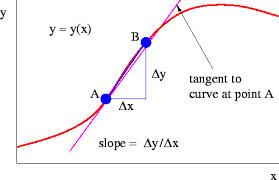
\includegraphics[height=.4\textheight]{derivative-definition.png}\\
	\hspace*{10pt}\hbox{\thinspace{\tiny\itshape labman.phys.uk.edu}}
\end{figure}

$f'(a)$ is the derivative of a function $f$ at $a$ if
$$f'(a) = \lim\limits_{x\to a} \frac{f(a+h)-f(a)}{h}$$

\vspace{6pt}

\textbf{Example:}
\begin{itemize}
	\item[(a)] Given $f(x)\frac{x}{2x-1}$ find $f'(a)$.
\end{itemize}
\end{frame}


\begin{frame}
\frametitle{\textbf{Derivative Laws}}
\begin{itemize}
	\item[1.] $f(x)=c \implies f'(x) = 0$
	\item[2.] $f(x) = x^n \implies f'(x) = nx^{n-1}$
	\item[3.] $F(x) = f(x)g(x) \implies F'(x)=f(x)g'(x) + g(x)f'(x)$
	\item[4.] $F(x) = \frac{f(x)}{g(x)} \implies F'(x)= \frac{g(x)f'(x)-f(x)g'(x)}{[g(x)]^2} \mbox{ if } g(x) \neq 0$
	\item[5.] $F(x) = f(x) + g(x) \implies f'(x) + g'(x)$
	\item[6.] $F(x)  = f(x) - g(x) \implies f'(x) - g'(x)$
	\item[7.] $f(x) = e^x \implies f'(x) = e^x$
	\item[8.] $f(x) = \log(x) \implies f'(x) = 1/x$
\end{itemize}

\vspace{6pt}

\textbf{Examples:}

Find the derivative of the following functions
\begin{itemize}
	\item[(a)] $f(t)=\frac{6}{\sqrt[3]{t^5}}$
	\item[(b)] $f(x)=\frac{x}{x+c/x}$
\end{itemize}
\end{frame}

\begin{frame}
\frametitle{\textbf{Using Derivatives to Find Max \& Min}}
Let $F$ be a function of $x$ and $A$ a set of numbers contained on the domain of $F$. 
\begin{itemize}
	\item[(i)] A point $x$ in $A$ is a maximum for $F$ on $A$ if $F(x) \geq F(y)$ for every $y$ on $A$. $F(x)$ is called the maximum of $F$ on $A$.
	\item[(ii)] A point $x$ in $A$ is a minimum for $F$ on $A$ if $F(x) \leq F(y)$ for every $y$ on $A$. $F(x)$ is called the minimum of $F$ on $A$.
\end{itemize}

\begin{theorem}
	Let $F$ be any function defined on $(a,b)$. If $x$ is a max or min point for $F$ on $(a,b)$ and $F$ is differentiable, then $F'(x)=0$
\end{theorem}
\end{frame}

\begin{frame}
\frametitle{\textbf{Using Derivatives to Find Max \& Min}}
A critical or stationary point of a function $F$ is a number $x$ such that $F'(x)=0$. $F(x)$ itself is called the critical value of $F$.

\vspace{6pt}
\textbf{Finding a Max or Min}\\
Consider a function on a closed interval $[a,b]$. In order to locate the max and/or min three kinds of points must be considered.
\begin{itemize}
	\item[1.]The critical points of $F$ in $[a,b]$.
	\item[2.]The end points of $[a,b]$.
	\item[3.]The points in $[a,b]$ such that $F$ is not differentiable at $x$.
\end{itemize}

\vspace{6pt}
\textbf{Examples:}\\
Find the max and min of each of the following
\begin{itemize}
	\item[(a)]
	\item[(b)]
	\item[(c)]
\end{itemize}
\end{frame}

\begin{frame}
\frametitle{\textbf{Rolle's Theorem}}
\begin{figure}
	\centering
	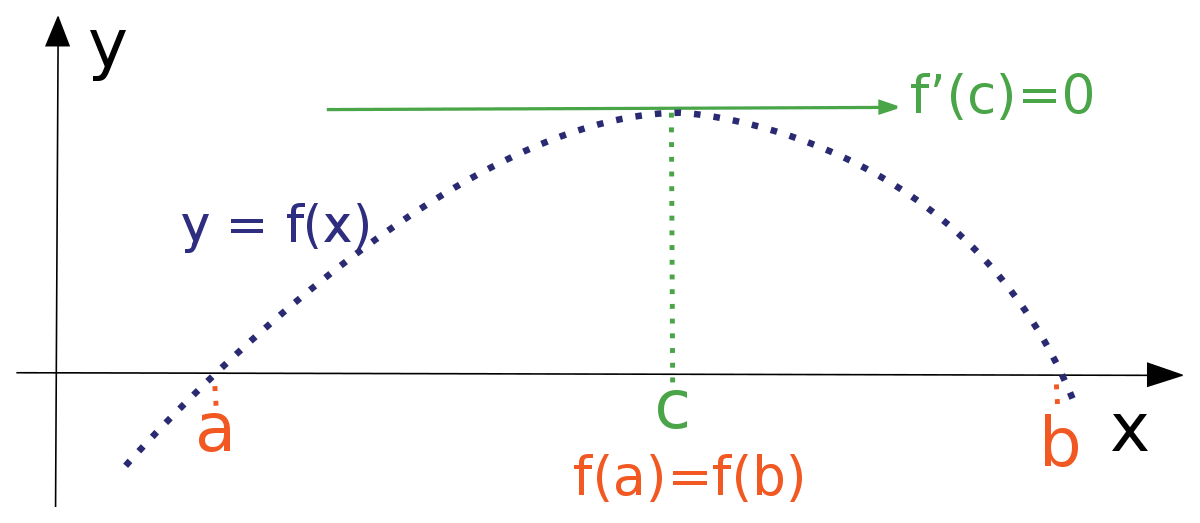
\includegraphics[height=.4\textheight]{rolles.png}\\
	\hspace*{10pt}\hbox{\thinspace{\tiny\itshape wikipedia}}
\end{figure}

\begin{theorem}[Rolle's Theorem]
	If $F$ is continuous on $[a,b]$ and differentiate on $(a,b)$ and $F(a)=F(b)$ then there is a number $x$ in $(a,b)$ such that $F'(x)=0$.
\end{theorem}
\end{frame}

\begin{frame}
\frametitle{\textbf{Mean Value Theorem}}
\begin{figure}
	\centering
	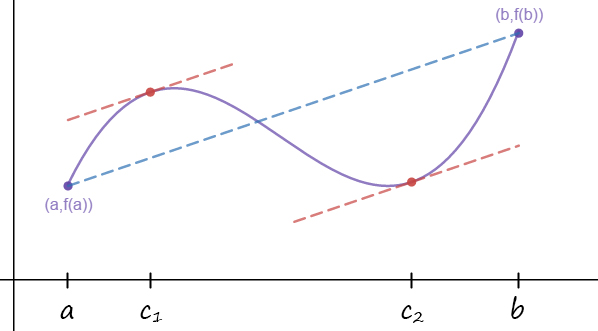
\includegraphics[height=.35\textheight]{meanvalue.jpg}\\
	\hspace*{10pt}\hbox{\thinspace{\tiny\itshape expii}}
\end{figure}
\begin{theorem}[Mean Value Theorem]
	If $F$ is continuous on $[a,b]$ and differentiable on $(a,b)$ then there is a number in $(a,b)$ such that
	$$F'(x) = \frac{F(b)-F(a)}{b-a}$$
\end{theorem}
\end{frame}

\begin{frame}
\frametitle{\textbf{Cauchy Mean Value Theorem}}

\begin{theorem}[Cauchy Mean Value Theorem]
	If $F$ and $g$ are continuous on $[a,b]$ and differentiable on $(a,b)$ then there is a number $x$ in $(a,b)$ such that
	$$\frac{F'(x)}{g'(x)} = \frac{F(b)-F(a)}{g(b)-g(a)} \implies [F(b)-F(a)]g'(x) = [g(b)-g(a)]F'(x)$$
\end{theorem}
\end{frame}


\begin{frame}
\frametitle{\textbf{L'Hopitals Rule}}
\begin{theorem}[L'Hopitals Rule]
	Suppose that $\lim\limits_{x \to a} F(x)=0$ and $\lim\limits_{x \to a} g(x)=0$ and
	\begin{itemize}
		\item[(i)] $F'$ and $g'$ exist for each $x$ of an interval about $x=a$ except possibly $a$ itself.
		\item[(ii)] $g'\neq0$ for $x\neq a$ in this interval.
		\item[(iii)] $\lim\limits_{x \to a} \frac{F'(x)}{g'(x)}=A$
	\end{itemize}
Then $\lim\limits_{x \to a} \frac{F(x)}{g(x)}=A$.
\end{theorem}
\vspace{6pt}
\textbf{Example:}
\begin{itemize}
	\item[(a)] $\lim\limits_{x\to 0} \frac{e^x-1}{\ln(1+x)}$
\end{itemize}
\end{frame}

%\begin{frame}
%\frametitle{What is a Limit?}
%\begin{figure}
%	\centering
%	\begin{subfigure}{0.48\textwidth}
%		
%		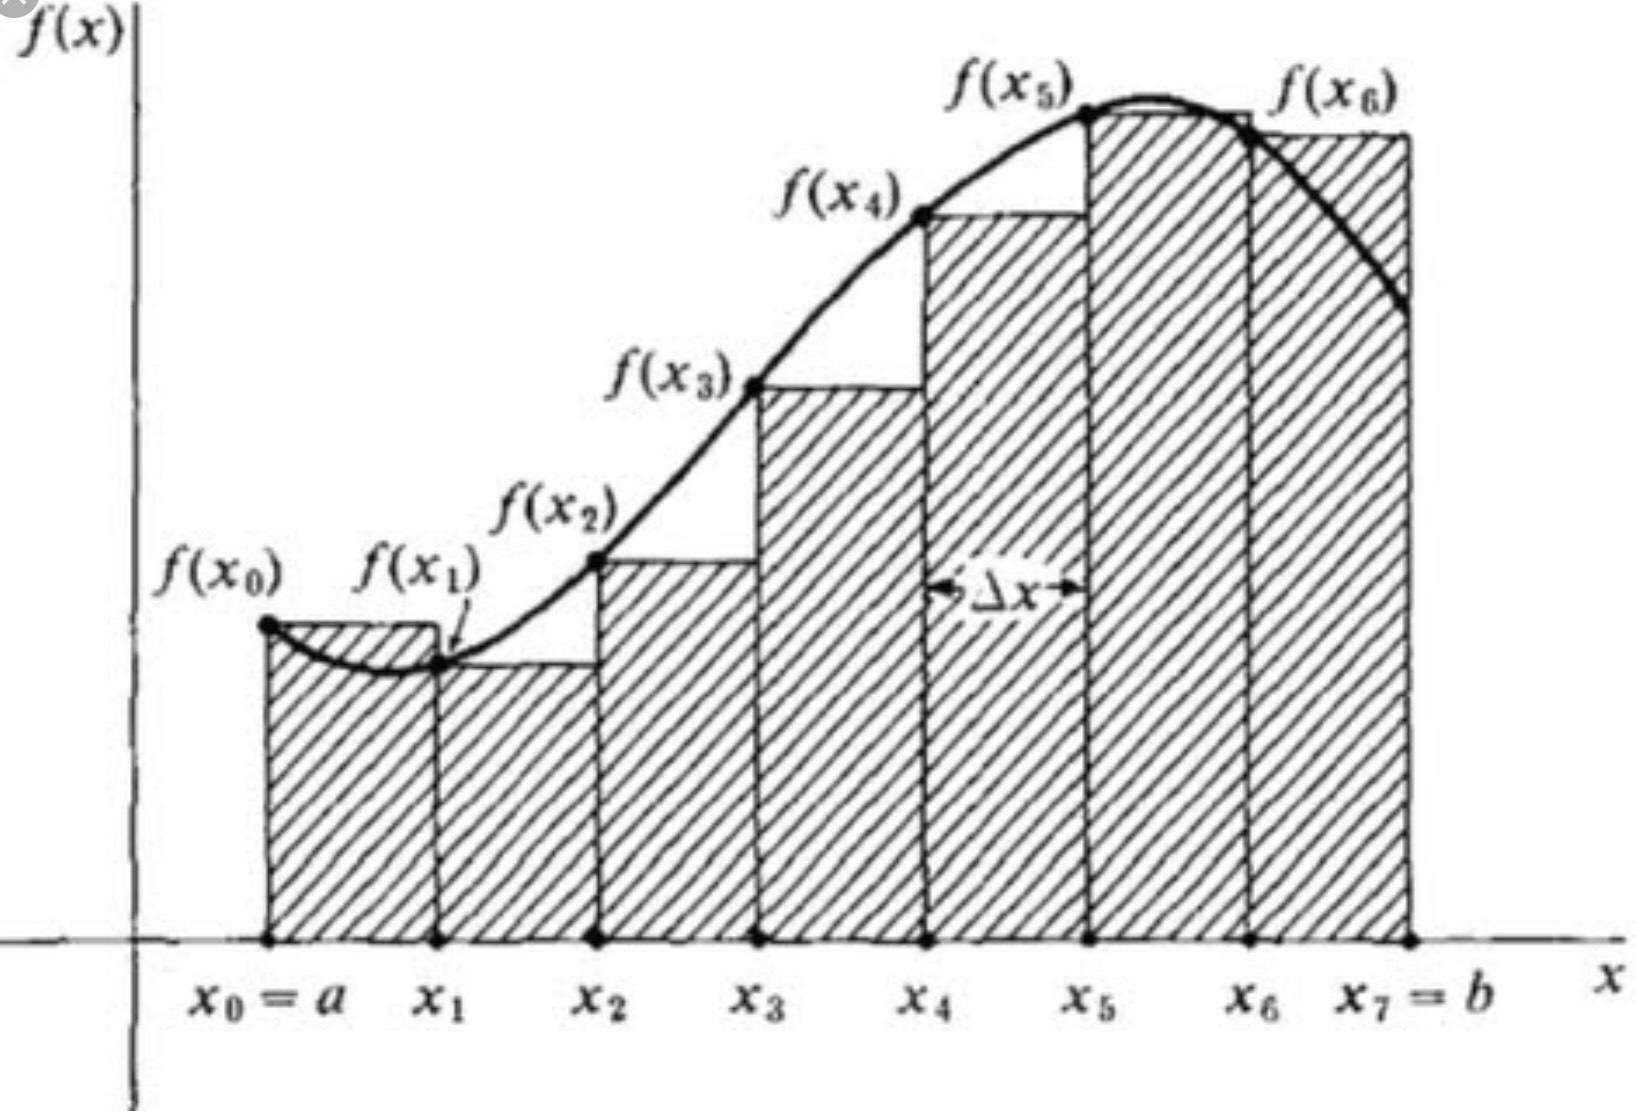
\includegraphics[width=\textwidth]{IMG_0380.jpg}
%		\hspace*{10pt}\hbox{\thinspace{\tiny\itshape vias.org}}
%		\caption{Single integration}
%	\end{subfigure}% 
%	~ 
%	\begin{subfigure}{0.48\textwidth}
%		
%		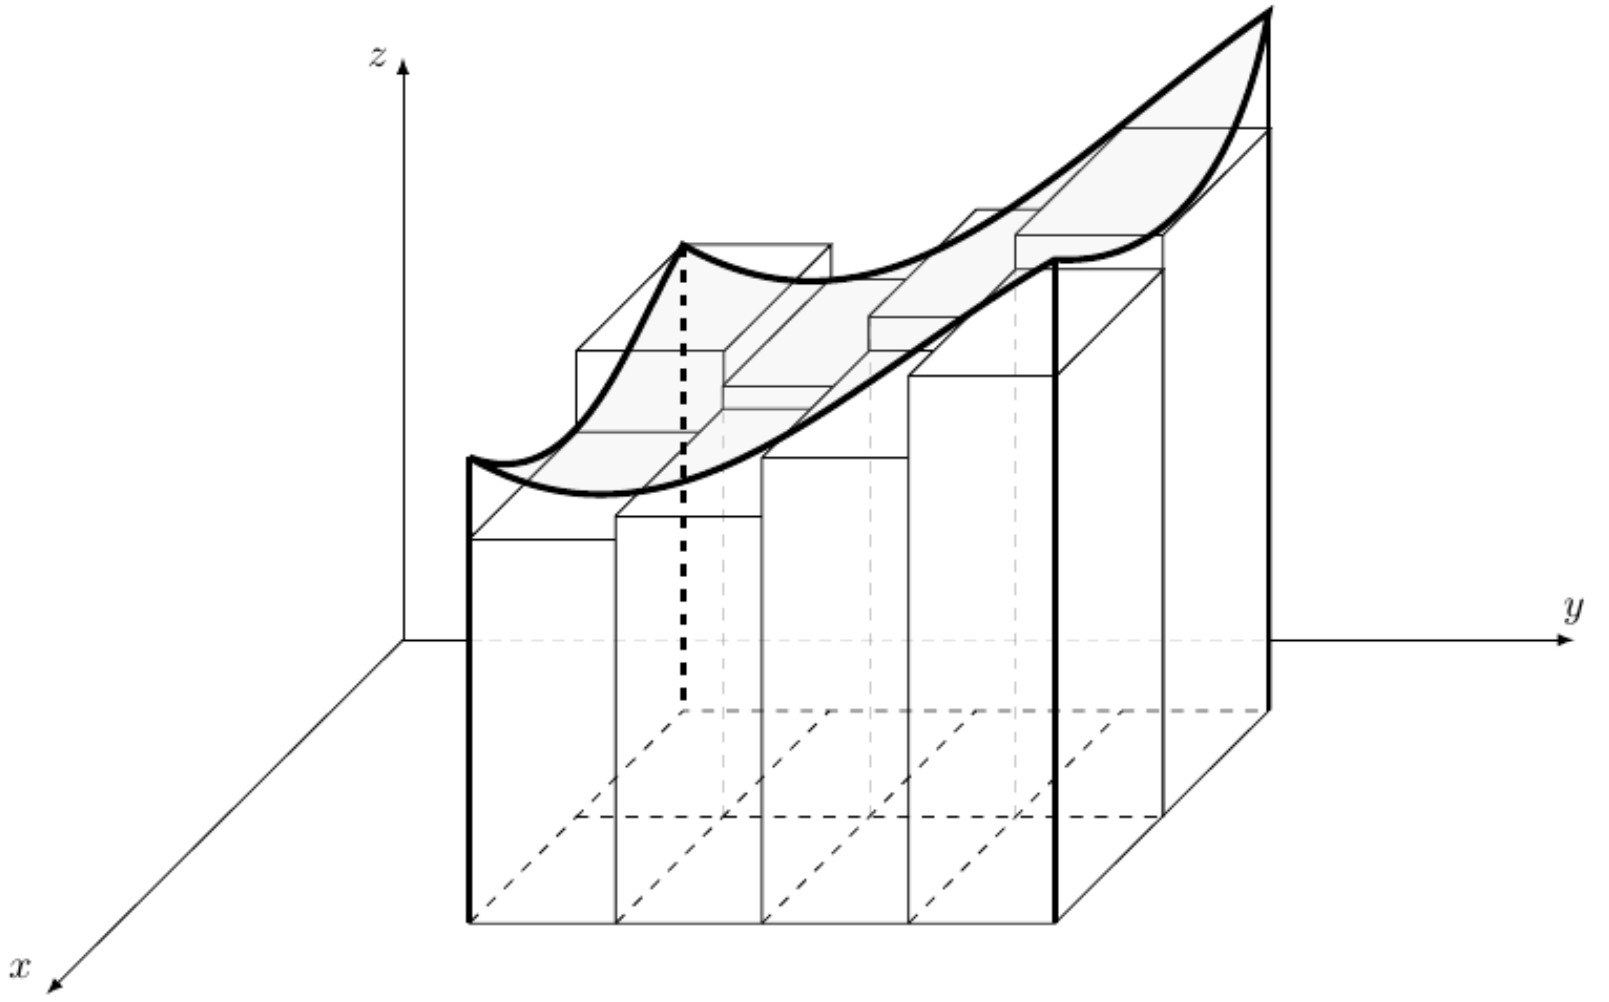
\includegraphics[width=\textwidth]{IMG_0385.jpg}
%		\hspace*{10pt}\hbox{\thinspace{\tiny\itshape tex.stackexchange.com}}
%		\caption{Double integration.}
%		\label{fig:2}
%	\end{subfigure}
%\end{figure}
%
%\end{frame}
%
%
%\begin{frame}
%\frametitle{Triple Integral}
%\begin{figure}
%	\centering
%	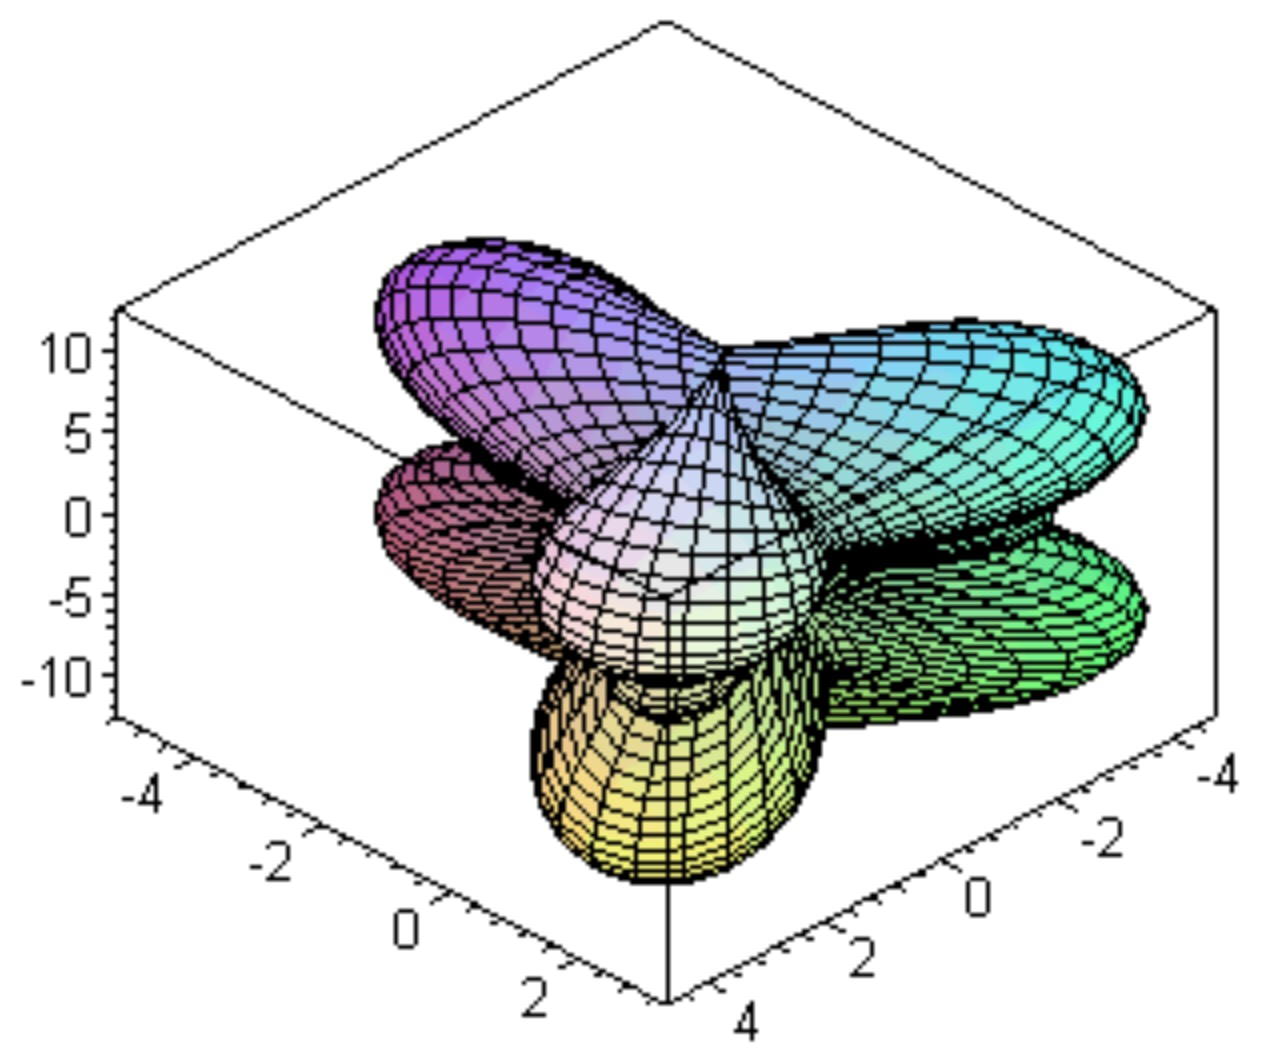
\includegraphics[height=.45\textheight]{IMG_0384.jpg}\\
%	\hspace*{10pt}\hbox{\thinspace{\tiny\itshape maplesoft.com}}
%\end{figure}
%
%$$\iiint\limits_{\mathbb{R}} F(x,y,z) dV = \int_{x=a}^{x=b} \int_{y=y_1(x)}^{y=y_2(x)} \int_{z=z_1(x,y)}^{z=z_2(x,y)} F(x,y,z) dz\,dy\,dx$$
%\textbf{Example:}
%\begin{itemize}
%	\item[(a)] $\int_0^1 \int_0^{1-x} \int_0^{2-x} xyz \,dz\,dy\,dx$
%\end{itemize}
%\end{frame}

\end{document}
